%%
\chapter{Design time details}
%%

Before the monitoring components can be generated and deployed we must design the system. First the metamodel must be designed, and after the metamodel is specified, we define graph queries, as they depend on the metamodel of the graph on which they are evaluated. These two steps can be done using EMF and Viatra eclipse technologies. \todo{ezt kicsit pontosítani, kifejteni}. 
 
In this chapter, I present how the monitoring components are generated from this these artifacts. 


\section{Generating classes from the metamodel}

The types of the metamodel are mapped to \cpp{} classes in the following way: From each type we generate three \cpp{} classes:

\begin{enumerate}
	\item An interface which provides access to an object of the type
	\item A local class, that stores the attributes and references of the instances allocated to the local computing unit.
	\item A proxy class, which can be used to substitute remote objects in references to them.
\end{enumerate}


\section{Overview of the query compilation workflow}

The compilation of the queries of the CPS is depicted in fig. \ref{figure:query-compile-workflow}. First the local search planner of the \viatra{} system creates a plan. We complete the generated plan with types and other supplementary information, and make a distributed version of the plans. After that, we use additional optimization specialized for our execution mechanism to improve the execution. After the fully optimized plan is ready, we can construct the generator model describing the source code structure and generate the \cpp{} files.

\begin{figure}[h]
	\begin{center}
		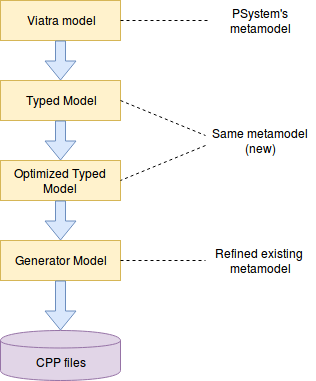
\includegraphics[width=0.5\textwidth]{figures/workflow.png}
		\caption{Query comompilation workflow}
		\label{figure:query-compile-workflow}
	\end{center}
\end{figure}


\section{Viatra plan}


\section{Completed plan}


\section{Additional optimization}


\section{C++ code generation}


